%%%%%%%%%%%%
%
% $Autor: Theilmann $
% $Datum: 04.04.2024 $
% $Pfad: DemonstratorSchrittmotor\Manual\Chapters\de\BEDFront.tex $
% $Version: 1 $
% !TeX spellcheck = en_GB/de_DE
% !TeX encoding = utf8
% !TeX root = manual 
% !TeX TXS-program:bibliography = txs:///BibTex
%
%%%%%%%%%%%%

\chapter{Elemente auf der Frontblende}
\begin{center}
	
	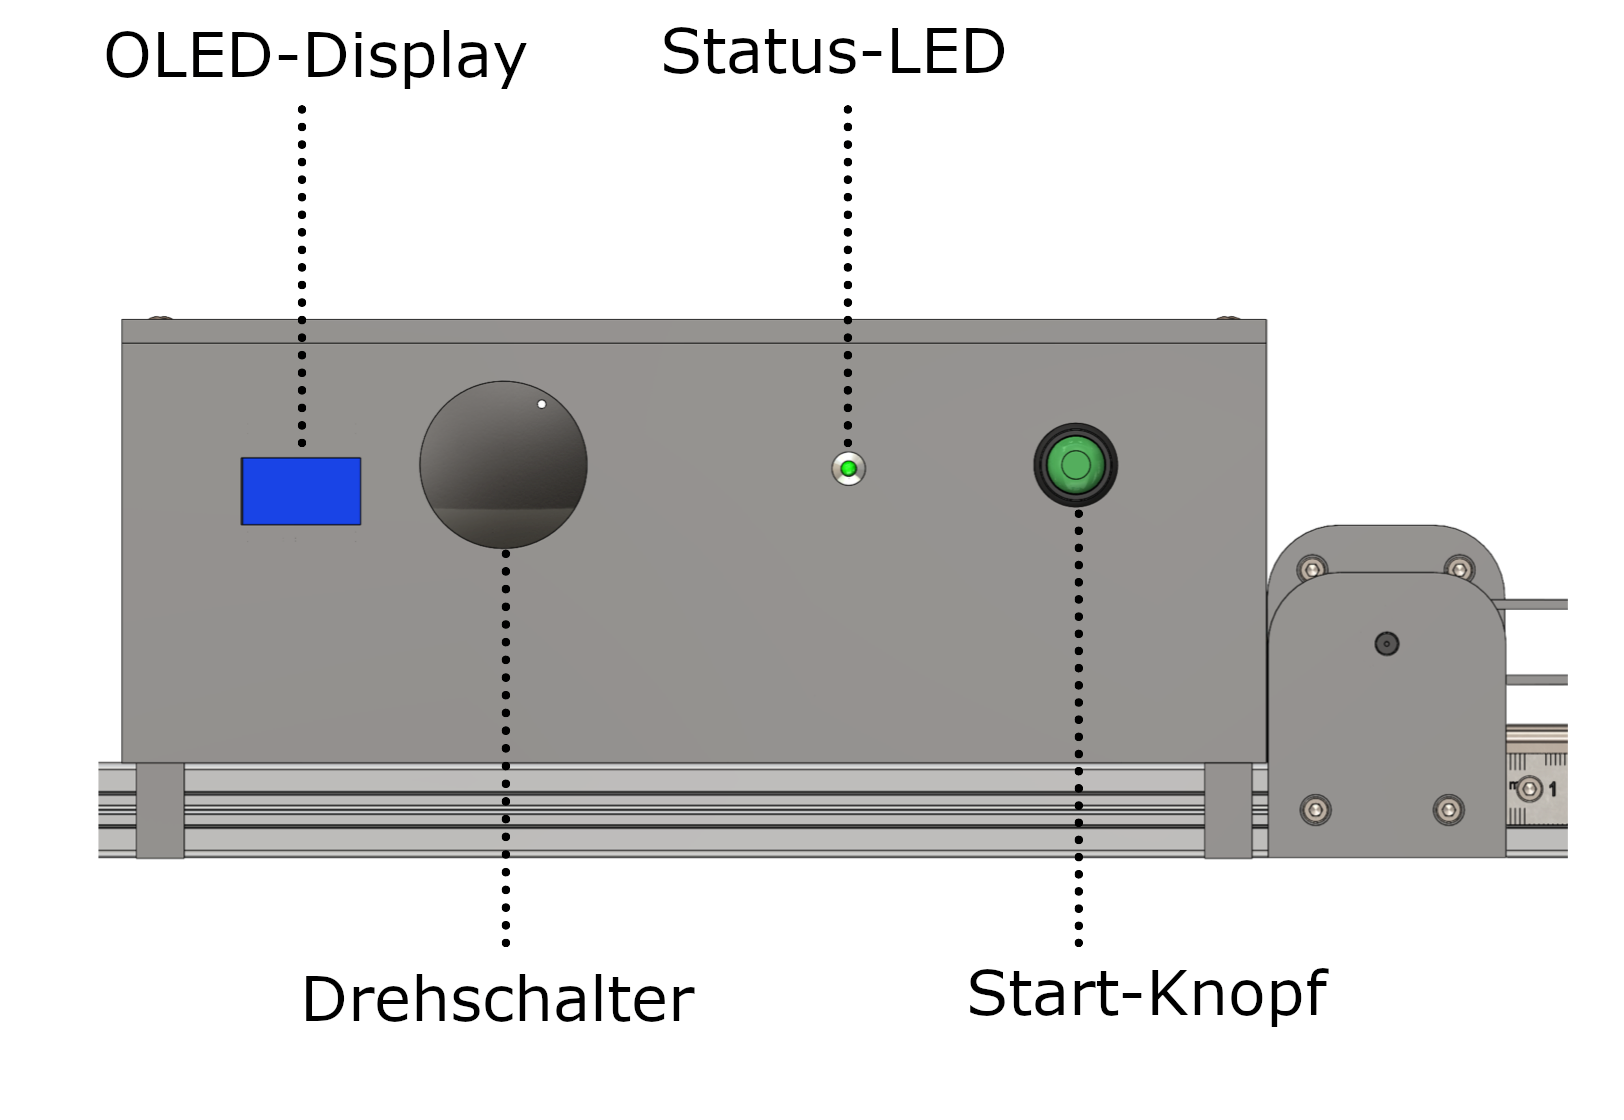
\includegraphics[width=\textwidth]{Images/Konstruktion2.png}
	%	\caption{Dies ist eine Konzeptskizze und wird noch ausgetauscht} \label{-}
\end{center}

	\textbf{OLED-Display}: 
\begin{itemize}
	\item Zeigt die aktuell ausgewählte Bewegungsstufe und den Status an
\end{itemize}

	\textbf{Status LED}: 
\begin{itemize}
	\item Zeigt den Status des Demonstrators an
\end{itemize}

	\textbf{Drehschalter}: 
\begin{itemize}
	\item Auswahl der Bewegungsstufe (detaillierte Einführung im Abschnitt \ref{STU} \nameref{STU})
\end{itemize}

	\textbf{Start-/Stopp-Taster}: 
\begin{itemize}
	\item Starten und stoppen der ausgewählten Bewegungsstufe
\end{itemize}
